\section{Spørgsmål 5}

\subsection{Fokuspunkter}
\begin{itemize}
	\item Hvad er normalisering og hvorfor bruges normalisering?
	\item Kom bla. ind på begrebet funktionelle afhængigheder.
	\item Samt redegør kort for normalformerne fra 1 til 4 Normalform (1..4NF)
\end{itemize}

\subsection{Litteratur}
\begin{itemize}
	
	\item Fra teori: Database Modeling and Design. Logical Design 5'th Ed.
	\begin{itemize}
		\item Kap. 6 (s. 109 - 130, ekstensivt s. 117 - 128).
	\end{itemize}
	
	\item Fra Database eLearning: \url{http://db.grussell.org/index.html}.
	\begin{itemize}
		\item Normalisation.
		\begin{itemize}
			\item Normalisation 0NF-3NF.
			\item Normalisation BCNF and Example.
		\end{itemize}
	\end{itemize}
	
	\item Fra wikipedia:
	\begin{itemize}
		\item \href{https://en.wikipedia.org/wiki/Database_normalization}{Database normalization}
		\begin{itemize}
			\item \url{http://en.wikipedia.org/wiki/Fourth_normal_form}
		\end{itemize}
	\end{itemize}
%	
%	\item Fra Agile Data Home Page:
%	\begin{itemize}
%		\item 
%	\end{itemize}
\end{itemize}

\newpage

% must
\subsection{Hvad er normalisering og hvorfor bruges normalisering?}\label{sec:normal}
Normalisering er den process der organiserer data i en database. Processen omfatter oprettelse af tabeller og etablering af relationer mellem tabellerne i henhold til et sæt regler, Normalformerne. Normalisering foretages for at minimere data redundancy. Normalisering prøver at opnå isolation af data, således at man kan Delete, Inserte og Update på en enkelt tabel, hvorpå ændringerne propageres gennem resten af databasen vha. fremmednøgler.

I en ikke normaliseret database kan man støde på disse propblemer:

\begin{itemize}
	\item \textbf{Update Anomaly} - Samme information findes i flere records. Dette kan føre til inconsistancy i forbindelse med Update.
	\item \textbf{Insertion Anomaly} - Når information ikke kan gemmes. Eksempel på databasen nedenfor hvor Course Code ikke kan være NULL
		\begin{figure}
			\centering
			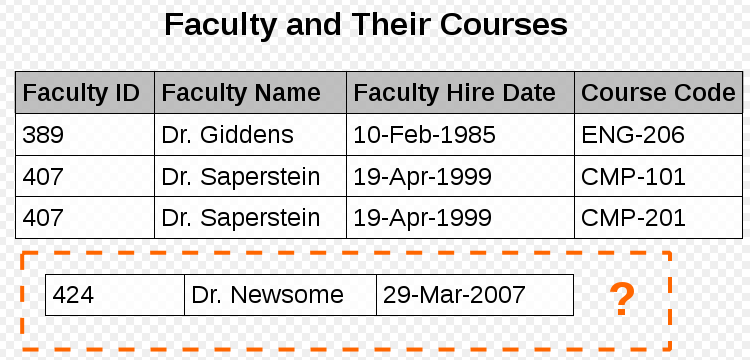
\includegraphics[width=0.7\linewidth]{figs/spm5/insertionAnomaly.PNG}
			\caption{Eksempel på insertion anomaly}
			\label{fig:insertionAnomaly}
		\end{figure}
	\item \textbf{Deletion Anomaly} - Når en tabel indeholder mere end én slags information. Eksemplet med fakultet og kurser, viser hvorledes Dr. Giddens forsvinder hvis man fjerner hans record.

	
\end{itemize}
% must
\subsection{Kom bla. ind på begrebet funktionelle afhængigheder}

% must
\subsection{Samt redegør kort for normalformerne fra 1 til 4 Normalform (1..4NF)}
